% \documentclass[table]{beamer}
\documentclass[table,handout]{beamer}
\setbeameroption{show notes}
% \setbeameroption{hide notes}
% \setbeameroption{show only notes}
\usepackage{varwidth}

\newif\ifhide
\newif\ifpost
\newif\ifhideclicker

% \hidetrue
% \hideclickertrue
% \posttrue

\newcommand{\whiteout}[1]{\textcolor{white}{#1}}
% \newcommand{\whiteoutbox}[1]{\fcolorbox{white}{white}{\parbox{\dimexpr \linewidth-2\fboxsep-2\fboxrule}{\whiteout{#1}}}}
% \newcommand{\notebox}[1]{\fcolorbox{blue}{white}{\parbox{\dimexpr \linewidth-2\fboxsep-2\fboxrule}{#1}}}
\newcommand{\whiteoutbox}[1]{\fcolorbox{white}{white}{\parbox{\linewidth}{\whiteout{#1}}}}
\newcommand{\notebox}[1]{\fcolorbox{blue}{white}{\parbox{\linewidth}{#1}}}
\newcommand{\blankbox}[1]{\phantom{\varwidth{\linewidth}\whiteoutbox{#1}\endvarwidth}}
\newcommand{\blank}[1]{\phantom{\varwidth{\linewidth}#1\endvarwidth}}

\ifhide%
    \newcommand{\hmask}[1]{\blank{#1}}%
\else%
    \newcommand{\hmask}[1]{#1}%
\fi

\ifhide%
    \newcommand{\wout}[1]{\whiteout{#1}}%
\else%
    \newcommand{\wout}[1]{#1}%
\fi

\ifhide%
    \newcommand{\hignore}[1]{}%
\else%
    \newcommand{\hignore}[1]{#1}%
\fi

\ifpost%
    \newcommand{\nopost}[1]{}%
\else%
    \newcommand{\nopost}[1]{#1}%
\fi

\ifhideclicker%
    \newcommand{\clickerslide}[1]{\stepcounter{clickerQuestionCounter}%
        \begin{frame}[t]
            \textcolor{blue}{Q \arabic{clickerQuestionCounter}:}
        \end{frame}}
\else%
    \newcommand{\clickerslide}[1]{#1}%
\fi

\ifhide%
    \newcommand{\hidebox}[1]{\blank{#1}}%
\else%
    \newcommand{\hidebox}[1]{\notebox{#1}}%
\fi

\ifhide%
    \newcommand{\wbox}[1]{\whiteoutbox{#1}}%
\else%
    \newcommand{\wbox}[1]{\notebox{#1}}%
\fi

\ifhide%
    \newcommand{\nbox}[1]{\blankbox{#1}}%
\else%
    \newcommand{\nbox}[1]{\notebox{#1}}%
\fi

\ifhideclicker%
    \newcommand{\clickeranswer}[1]{#1}%
\else%
    \ifhide%
        \newcommand{\clickeranswer}[1]{#1}%
    \else%
        \newcommand{\clickeranswer}[1]{\textbf{\textcolor{blue}{#1}}}%
    \fi
\fi

\usepackage{beamerthemesplit}
% \usetheme{boxes}
\usetheme{Malmoe}
\usecolortheme{seahorse}
% \usecolortheme{seagull}
\usepackage{ifthen}
\usepackage{xspace}
\usepackage{multirow}
\usepackage{multicol}
\usepackage{booktabs}
\usepackage{xcolor}
\usepackage{wasysym}
\usepackage{comment}
\usepackage{hyperref}
\hypersetup{pdfborder={0 0 0}, colorlinks=true, urlcolor=blue, linkcolor=blue, citecolor=blue}
\usepackage{changepage}
\usepackage[compatibility=false]{caption}
\captionsetup[figure]{font=scriptsize, labelformat=empty, textformat=simple, justification=centering, skip=2pt}
\usepackage{tikz}
\usetikzlibrary{trees,calc,backgrounds}

\usepackage[bibstyle=joaks-slides,maxcitenames=3,mincitenames=1,backend=biber]{biblatex}

\newrobustcmd*{\shortfullcite}{\AtNextCite{\renewbibmacro{title}{}\renewbibmacro{in:}{}\renewbibmacro{number}{}}\fullcite}

\newrobustcmd*{\footlessfullcite}{\AtNextCite{\renewbibmacro{title}{}\renewbibmacro{in:}{}}\footfullcite}

% Make all footnotes smaller
% \renewcommand{\footnotesize}{\scriptsize}

\definecolor{myGray}{gray}{0.9}
\colorlet{rowred}{red!30!white}

\setbeamertemplate{blocks}[rounded][shadow=true]

\setbeamercolor{defaultcolor}{bg=structure!30!normal text.bg,fg=black}
\setbeamercolor{block body}{bg=structure!30!normal text.bg,fg=black}
\setbeamercolor{block title}{bg=structure!50!normal text.bg,fg=black}

\newenvironment<>{varblock}[2][\textwidth]{%
  \setlength{\textwidth}{#1}
  \begin{actionenv}#3%
    \def\insertblocktitle{#2}%
    \par%
    \usebeamertemplate{block begin}}
  {\par%
    \usebeamertemplate{block end}%
  \end{actionenv}}

\newenvironment{displaybox}[1][\textwidth]
{
    \centerline\bgroup\hfill
    \begin{beamerboxesrounded}[lower=defaultcolor,shadow=true,width=#1]{}
}
{
    \end{beamerboxesrounded}\hfill\egroup
}

\newenvironment{onlinebox}[1][4cm]
{
    \newbox\mybox
    \newdimen\myboxht
    \setbox\mybox\hbox\bgroup%
        \begin{beamerboxesrounded}[lower=defaultcolor,shadow=true,width=#1]{}
    \centering
}
{
    \end{beamerboxesrounded}\egroup
    \myboxht\ht\mybox
    \raisebox{-0.25\myboxht}{\usebox\mybox}\hspace{2pt}
}

\newenvironment{mydescription}{
    \begin{description}
        \setlength{\leftskip}{-1.5cm}}
    {\end{description}}

\newenvironment{myitemize}{
    \begin{itemize}
        \setlength{\leftskip}{-.3cm}}
    {\end{itemize}}

% footnote without a marker
\newcommand\barefootnote[1]{%
  \begingroup
  \renewcommand\thefootnote{}\footnote{#1}%
  \addtocounter{footnote}{-1}%
  \endgroup
}

% define formatting for footer
\newcommand{\myfootline}{%
    {\it
    \insertshorttitle
    \hspace*{\fill} 
    \insertshortauthor, \insertshortinstitute
    % \ifx\insertsubtitle\@empty\else, \insertshortsubtitle\fi
    \hspace*{\fill}
    \insertframenumber/\inserttotalframenumber}}

% set up footer
\setbeamertemplate{footline}{%
    \usebeamerfont{structure}
    \begin{beamercolorbox}[wd=\paperwidth,ht=2.25ex,dp=1ex]{frametitle}%
        % \Tiny\hspace*{4mm}\myfootline\hspace{4mm}
        \tiny\hspace*{4mm}\myfootline\hspace{4mm}
    \end{beamercolorbox}}

% remove navigation bar
\beamertemplatenavigationsymbolsempty

\makeatletter
    \newenvironment{noheadline}{
        \setbeamertemplate{headline}[default]
        \def\beamer@entrycode{\vspace*{-\headheight}}
    }{}
\makeatother

\newcounter{clickerQuestionCounter}
\ifhideclicker%
\newenvironment{clickerquestion}
{ \stepcounter{clickerQuestionCounter}
  \begin{enumerate}[Q \arabic{clickerQuestionCounter}:]\color{white} }
{ \end{enumerate} }
\else%
\newenvironment{clickerquestion}
{ \stepcounter{clickerQuestionCounter}
  \begin{enumerate}[Q \arabic{clickerQuestionCounter}:] }
{ \end{enumerate} }
\fi

\ifhideclicker%
\newenvironment{clickeroptions}
{ \begin{enumerate}[\begingroup\color{white} 1)\endgroup]\color{white} }
{ \end{enumerate} }
\else%
\newenvironment{clickeroptions}
{ \begin{enumerate}[\begingroup\color{red} 1)\endgroup] }
{ \end{enumerate} }
\fi


\tikzstyle{centered} = [align=center, text centered, font=\sffamily\bfseries]
\tikzstyle{skip} = [centered, inner sep=0pt, fill]
\tikzstyle{empty} = [centered, inner sep=0pt]
\tikzstyle{inode} = [centered, circle, minimum width=4pt, fill=black, inner sep=0pt]
\tikzstyle{tnode} = [centered, circle, inner sep=1pt]
\tikzset{
  % edge styles
  level distance=10mm,
  mate/.style={edge from parent/.style={draw,distance=3pt}},
  mleft/.style={grow=left, level distance=10mm, edge from parent path={(\tikzparentnode.west)--(\tikzchildnode.east)}},
  mright/.style={grow=right, level distance=10mm, edge from parent path={(\tikzparentnode.east)--(\tikzchildnode.west)}},
  % node styles
  male/.style={rectangle,minimum size=4mm,fill=gray!80},
  female/.style={circle,minimum size=4mm,fill=gray!80},
  amale/.style={male,fill=red},
  afemale/.style={female,fill=red},
}

\newcommand{\highlight}[1]{\textcolor{violet}{\textit{\textbf{#1}}}}
\newcommand{\super}[1]{\ensuremath{^{\textrm{\sffamily #1}}}}
\newcommand{\sub}[1]{\ensuremath{_{\textrm{\sffamily #1}}}}
\newcommand{\dC}{\ensuremath{^\circ{\textrm{C}}}}
\newcommand{\tb}{\hspace{2em}}
\providecommand{\e}[1]{\ensuremath{\times 10^{#1}}}
\newcommand{\myHangIndent}{\hangindent=5mm}

\newcommand{\spp}[1]{\textit{#1}}

\newcommand\mybullet{\leavevmode%
\usebeamertemplate{itemize item}\hspace{.5em}}

\makeatletter
\newcommand*{\rom}[1]{\expandafter\@slowromancap\romannumeral #1@}
\makeatother

\newcommand{\blankslide}{{\setbeamercolor{background canvas}{bg=black}
\setbeamercolor{whitetext}{fg=white}
\begin{frame}<handout:0>[plain]
\end{frame}}}

\newcommand{\whiteslide}{
\begin{frame}<handout:0>[plain]
\end{frame}}

\newcommand{\f}[1]{\ensuremath{F_{#1}}}
\newcommand{\x}[1]{X\ensuremath{^{#1}}}
\newcommand{\y}[1]{Y\ensuremath{^{#1}}}

% Population growth macros
\newcommand{\popsize}[1]{\ensuremath{N_{#1}}}
\newcommand{\popgrowthratediscrete}[1]{\ensuremath{\lambda_{#1}}}
\newcommand{\popgrowthrate}[1]{\ensuremath{r_{#1}}}
\newcommand{\ptime}{\ensuremath{t}\xspace}

\tikzset{hide on/.code={\only<#1>{\color{white}}}}
\tikzset{
    invisible/.style={opacity=0},
    visible on/.style={alt={#1{}{invisible}}},
    alt/.code args={<#1>#2#3}{%
        \alt<#1>{\pgfkeysalso{#2}}{\pgfkeysalso{#3}}
        % \pgfkeysalso doesn't change the path
    },
}

% \bibliography{../bib/references}
\bibliography{references}
\author[J.\ Oaks]{
    %Jamie R.\ Oaks\inst{1}
    Jamie R.\ Oaks
}
\institute[BIOL 180]{
    \inst{}%
        BIOL 180: Introductory Biology
}



\title[Human Genetic Disease]{Human Genetic Disease}
% \date{\today}
\date{April 13, 2015}

\begin{document}

\begin{noheadline}
\maketitle
\end{noheadline}

\nopost{
\begin{noheadline}
\begin{frame}[c]
    \vspace{-6mm}
    \begin{center} 
        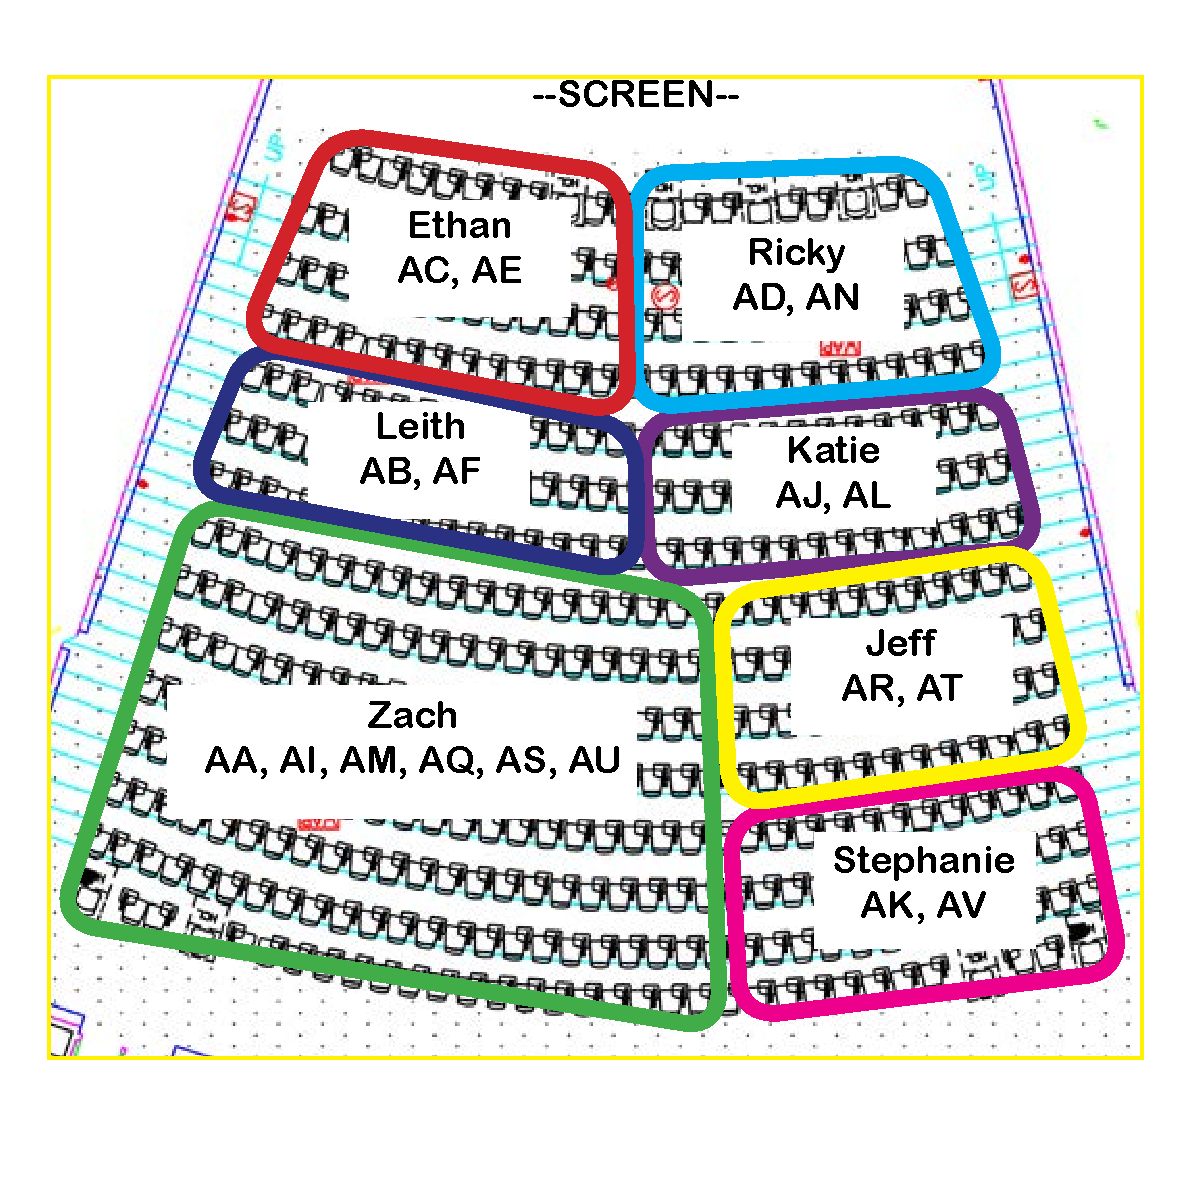
\includegraphics[height=1.3\textheight]{../images/seating-chart.pdf}
    \end{center}
\end{frame}
\end{noheadline}
}

\clickerslide{
\begin{noheadline}
\begin{frame}
    \begin{clickerquestion}
        \item Why have eugenics programs in humans been unsuccessful? 
        \begin{clickeroptions}
            \item \clickeranswer{These programs remove variation from the
                    population, and thus decrease the ability of the population
                    to respond to selection pressures.}
            \item \clickeranswer{More closely related individuals are more
                    likely to carry the same deleterious recessive alleles, and
                    thus their offspring are more likely to express genetic
                    disease caused by such alleles.}
            \item \clickeranswer{The environment (and selection pressures) is
                    always changing, and so there are no traits that will be
                    universally ``better'' than others.}
            \item \clickeranswer{These programs often select for
                    environmentally determined traits.}
        \end{clickeroptions}
    \end{clickerquestion}

    \note[item]{Eugenics pre-dated natural selection (e.g., castrating the
        insane and homosexuals)}
    \note[item]{Side-note: Alan Turing (1952; chemically castrated)}
    \note[item]{Francis Galton (Darwin's half cousin) coined term in 1883 (1
        year after Darwin's death)}
    \note[item]{Big in early 1900s (funding, international conferences, etc.)}
    \note[item]{Fell out of favor in 1930s; Why? Nazi's AND modern synthesis!}
\end{frame}
\end{noheadline}
}

\begin{noheadline}
\begin{frame}
\frametitle{Today's issues:}
\tableofcontents
\end{frame}
\end{noheadline}


\section{Transmission genetics of human disease}

\begin{frame}
    \uncover<1->{
    Many (or most) recessive alleles have loss-of-function or knock-out
    mutations---they do not produce a functional product.
    }

    \uncover<2->{
    \begin{itemize}
        \item If a recessive allele is loss-of-function, why do heterozygotes
            have a normal phenotype? 

            \nbox{The ``normal'' copy of the gene can produce enough
                protein for normal functioning of cells.}

        \item What does it mean to say that deleterious recessives ``hide out''
            (from natural selection) in heterozygotes? 

            \nbox{Selection acts on \highlight{phenotypes}, so the
                allele is ``invisible'' to selection.}
    \end{itemize}
    }
\end{frame}

\clickerslide{
\begin{frame}
    \begin{clickerquestion}
        \item Deleterious alleles have low fitness in the current environment
            and are eliminated by natural selection. Which of the following
            types of deleterious alleles are eliminated fastest, and which
            slowest? 
        \begin{clickeroptions}
            \item No difference among recessive, dominant, or co-dominant
                alleles.
            \item Co-dominant alleles are slowest, recessive alleles are
                medium, and dominant alleles are fastest.
            \item Co-dominant alleles are slowest, dominant alleles are medium,
                and recessive alleles are fastest.
            \item \clickeranswer{Recessive alleles are slowest, and dominant
                    and co-dominant alleles are faster and equal.}
        \end{clickeroptions}
    \end{clickerquestion}
\end{frame}
}

\clickerslide{
\begin{frame}
    \begin{clickerquestion}
        \item
        My friends L and D are both carriers for the genetic disease cystic
        fibrosis (CF), which is caused by autosomal recessive alleles.
        What proportion of their children are expected to have CF?
        \begin{clickeroptions}
            \item 0
            \item \clickeranswer{1/4}
            \item 0.5
            \item 3/4 
            \item 1.0
        \end{clickeroptions}
    \end{clickerquestion}
\end{frame}
}

\clickerslide{
\begin{frame}
    \begin{clickerquestion}
        \item
        Suppose that L has CF (is symptomatic) but D is unaffected and
        homozygous.
        What proportion of their children are expected to have CF?
        \begin{clickeroptions}
            \item \clickeranswer{0}
            \item 0.25
            \item 1/2
            \item 3/4 
            \item 1.0
        \end{clickeroptions}
    \end{clickerquestion}
\end{frame}
}

\clickerslide{
\begin{frame}
    \begin{centering}
    \begin{tikzpicture}[font=\footnotesize]
        % 1st Gen
        \node(G1M)[male,label=left: {Male}]{} 
            child[mright,mate]{coordinate(G1X1) child{node(G1F)[afemale,label=right: {Female}]{}}}
        ;
        % 2nd Generation
        \node at(G1X1){}
            [edge from parent fork down,sibling distance=10mm, level distance=15mm]
            child{node[female]{}
                child[mate,mleft]{coordinate(G2X1) child{node[male]{}}}
            }
            child{node[female]{}}
            child{node[male]{}}
            child{node[male]{}}
            child{node[male]{}
                child[mate,mright]{coordinate(G2X2) child{node(G2F3)[female]{}}}
            }
        ;
        % 3rd Generation
        \node at(G2X1){}
            [edge from parent fork down, sibling distance=10mm, level distance=15mm]
            child{node[amale]{}}
            child{node[female]{}}
            child{node[male]{}}
            child{node[female]{}}
        ;
        \node at(G2X2){}
            [edge from parent fork down, sibling distance=10mm, level distance=15mm]
            child{node[male]{}}
            child{node[female]{}}
            child{node[male]{}}
        ;
    \end{tikzpicture}
    \end{centering}

    \vspace{0.5cm}
    \begin{clickerquestion}
        \item
        Which of the following is most likely? 
        \begin{clickeroptions}
            \item The disease allele is X-linked and recessive.
            \item The disease allele is Y-linked. 
            \item \clickeranswer{The disease allele is autosomal and recessive.}
            \item Affected individuals have novel mutations; the disease
                    allele is autosomal dominant.
        \end{clickeroptions}
    \end{clickerquestion}
\end{frame}
}

\clickerslide{
\begin{frame}
    \begin{centering}
    \begin{tikzpicture}[font=\footnotesize]
        % 1st Gen
        \node(G1M)[amale,label=left: {Male}]{} 
            child[mright,mate]{coordinate(G1X1) child{node(G1F)[female,label=right: {Female}]{}}}
        ;
        % 2nd Generation
        \node at(G1X1){}
            [edge from parent fork down,sibling distance=10mm, level distance=15mm]
            child{node[afemale]{}
                child[mate,mleft]{coordinate(G2X1) child{node[male]{}}}
            }
            child{node[afemale]{}}
            child{node[afemale]{}}
            child{node[male]{}}
            child{node[male]{}}
            child{node[male]{}
                child[mate,mright]{coordinate(G2X2) child{node(G2F3)[female]{}}}
            }
        ;
        % 3rd Generation
        \node at(G2X1){}
            [edge from parent fork down, sibling distance=10mm, level distance=15mm]
            child{node[amale]{}}
            child{node[afemale]{}}
            child{node[male]{}}
            child{node[female]{}}
        ;
        \node at(G2X2){}
            [edge from parent fork down, sibling distance=10mm, level distance=15mm]
            child{node[male]{}}
            child{node[female]{}}
            child{node[male]{}}
        ;
    \end{tikzpicture}
    \end{centering}

    \vspace{0.5cm}
    \begin{clickerquestion}
        \item
        Which of the following is most likely? 
        \begin{clickeroptions}
            \item \clickeranswer{The disease allele is X-linked and dominant.}
            \item The disease allele is X-linked and recessive.
            \item The disease allele is autosomal and dominant.
            \item The disease allele is Y-linked and dominant. 
        \end{clickeroptions}
    \end{clickerquestion}
\end{frame}
}

\clickerslide{
\begin{frame}
    \begin{clickerquestion}
        \item
        A friend of mine has severe, juvenile-onset arthritis.
        There is NO history of the illness anywhere in her family or her
        husband's family, going back many generations.
        All three of her children (all are female) are also affected.
        Which of the following is most likely? 
        \begin{clickeroptions}
            \item The disease allele is X-linked and recessive.
            \item The disease allele is an autosomal recessive.
            \item \clickeranswer{The mom has a novel mutation; the disease
                    allele is autosomal dominant.}
            \item The disease allele is X-linked; the mom is homozygous. 
        \end{clickeroptions}
    \end{clickerquestion}
\end{frame}
}

\section{Selection dynamics of cystic fibrosis alleles}

\begin{frame}
    \begin{description}
        \item[Observation 1:]
            Alleles that cause cystic fibrosis (CF) are at a frequency of about
            2\% in populations of Northern European ancestry.
            Given the strength of selection against individuals with the
            disease phenotype, this is very high, even though the disease
            alleles are recessive.
        \item[Observation 2:]
            \emph{Salmonella typhi}, the bacteria that causes typhoid fever,
            enters gut cells through the normal CF gene product (CFTR protein).
            This event starts an infection.
    \end{description}
    \barefootnote{\shortfullcite{Pier1998}}
\end{frame}

\begin{frame}
    \begin{description}
        \item[Hypothesis:] \ \\
            \uncover<2->{Individuals who are heterozygous for the recessive CF
                disease allele are protected against typhoid fever.}

        \vspace{0.5cm}
        \item[Experiment:] \ \\
            \uncover<3->{Create mouse cells that have zero (homozygous
                dominant) one (heterozygous) and two (homozygous recessive)
                copies of the CFTR allele that causes CF, and expose them to
                \emph{S.\ typhi}.}
    \end{description}

    \begin{itemize}
        \item<4->{Why use mouse cells for the experiment instead of cells from
                humans that do and do not carry the CF allele?}
            \nbox{Any differences are due only to difference in presence of
                CFTR, not some other difference among of human cells}
    \end{itemize}
\end{frame}

\clickerslide{
\begin{frame}[t]
    \begin{columns}
        \column{.7\textwidth}
        \begin{uncoverenv}<2->
        \begin{clickerquestion}
            \item What do these results suggest?
            \begin{clickeroptions}
                \item The results support our hypothesis, because cells
                    that are homozygous for the recessive CF disease allele
                    are protected against \emph{S.\ typhi}.
                \item \clickeranswer{The results support our hypothesis,
                        because cells that are carriers for the recessive CF
                        disease allele are protected against \emph{S.\ typhi}.}
                \item The results do not support our hypothesis, because
                    cells that are heterozygous for the CF disease allele
                    are less protected against \emph{S.\ typhi} than
                    cells that have two copies of the allele.
                \item Our hypothesis was flawed, because individuals that are
                    heterozygous for the CF disease allele will have lower
                    fitness.
            \end{clickeroptions}
        \end{clickerquestion}
        \end{uncoverenv}
        \column{.36\textwidth}
        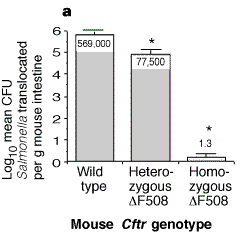
\includegraphics[height=4.2cm]{../images/pier-1998-histogram.png}
    \end{columns}

    \note[item]{Key: Note the log scale}
    \note[item]{Homozygous = 569,000}
    \note[item]{Heterozygous = 77,500}
    \note[item]{Homozygous mutant = 1.3}
    \note[item]{Is this the best way to graph these data?}
\end{frame}
}

\section{Selection on alleles associated with late-onset illness}

\begin{frame}
    Which should be more common, and why?

    \begin{enumerate}
        \item Alleles that contribute to Type 2 diabetes (adult onset)
        \item Alleles that contribute to Type 1 diabetes (juvenile onset)
    \end{enumerate}

    \nbox{Type 2: People can reproduce before becoming symptomatic, so there
        will be less selection against it.}
\end{frame}

\clickerslide{
\begin{frame}
    \begin{clickerquestion}
        \item Type 1 diabetes is treated with insulin injections. Which of the
            following statements is correct?
        \begin{clickeroptions}
            \item Because of better education, nutrition, and medical care,
                human populations are no longer evolving. 
            \item Because of better education, nutrition, and medical care,
                average fitness is decreasing in humans.
            \item Since insulin became widely available, alleles associated
                with type 1 diabetes have decreased in frequency.
            \item \clickeranswer{Since insulin became widely available, alleles
                    associated with type 1 diabetes have increased in
                    frequency.}
        \end{clickeroptions}
    \end{clickerquestion}
\end{frame}
}

\begin{frame}
    In terms of fitness, are human populations in the industrialized countries
    becoming ``weaker'' (individuals are less fit, on average), due to improved
    healthcare? 
    \nbox{I would argue ``no'', because (1) fitness is only meaningful
        within the context of the current environment, (2) having more
        variation in the population makes it more adaptable (more variation to
        respond to changing selection pressures).}
\end{frame}


\end{document}

